\def \secname {Introduction to Finite Difference Approximation (FDA)}

\section[\secname]{\hyperlink{toc}{\secname}}


\subsection{Basic Idea via simple example}
\begin{itemize}
    \item Suppose We are given velocity of particle

    \[ v(t) \equiv \frac{dx}{dt}\]

    \item  Can approximate velocity using 

    \[ v(t) \equiv \frac{dx}{dt} \approx \frac{x(t+\Delta t) - x(t)}{\Delta t}\]

    Some finite increment in time; as $\Delta t \rightarrow 0$, approximation becomes more accurate.

    \item Solve for $x(t+\Delta t)$

    \[ x(t+ \Delta t) \approx x(t) + \Delta t v(t) \]

    \item So, given x(0) can determine

    \[ x(\Delta t) = x(0) + \Delta t v(0)\]
    \[  x(2 \Delta t) =  x(\Delta t) + \Delta t v(\Delta t)\]
    \[  x(3 \Delta t) =  x(2 \Delta t) + \Delta v(2 \Delta t)\] \[...\]

    \item Illustrates 3 key steps in solving ODEs (PDEs) with FDA

    \begin{enumerate}
        \item \textbf{Replace} Continuous Independent variable, t, with discrete values $0,\Delta t, 2\Delta t, 3\Delta t, ...$
        \item \textbf{Discretization of Equations: Replace derivatives with FDAs}
        \item \textbf{Solution:} Solve algebraic equations for approximate solution. Values (Here, once an initial condition x(0) is given)
    \end{enumerate}
\end{itemize}

\subsection{Mathematical Preliminaries}

\subsubsection{Big-O Notation}

\begin{itemize}
    \item Definition: $f(h)$ is $O(h^p)$ (Note: $h$ think stepsize, $\ll 1$) if and only if there are two positive real numbers $M$ , $h_0$ such that 

    \[ |f(h)| \leq M|h^p| \qquad \text{for all } h\ h_0\]

    \[ O(h^2) > O(h^3)\]
\end{itemize}

\subsubsection{Taylor Series}

\begin{itemize}
    \item Taylor series and FDAs
    \begin{itemize}
        \item Can be used to derive FDAs
        \item Can be used to establish accuracy of FDAs (**)
    \end{itemize}
    \item Usually T.S. to expand expressions like $f(x+h)$ (h; expansion parameter) about $f(x)$

    \[ f(x+h) = \sum_{n=0}^\infty h^n \frac{f^{(n)}(x)}{n!} \qquad \text{TS}\]

    for nth derivative of f evaluated at x

    \[ f(x+h) = f(x) + hf'(x) + \frac{1}{2} h^2 f''(x) + \frac{1}{6} h^3 f'''(x) + O(h^4)\]
    \[ f(x-h) = f(x) - hf'(x) + \frac{1}{2} h^2 f''(x) - \frac{1}{6} h^3 f'''(x) + O(h^4)\]    
\end{itemize}

\subsubsection{Discretization: Step 1 : Finite Difference Grids (Meshes, Lattices)}

\begin{itemize}
    \item Physical Domain (Continuum)

    \[ x_{min} \leq x \leq x_{max}\]

    \[ 0 \leq t \leq t_{max}\]
    
    \item Uniform finite difference grid $x_j$

    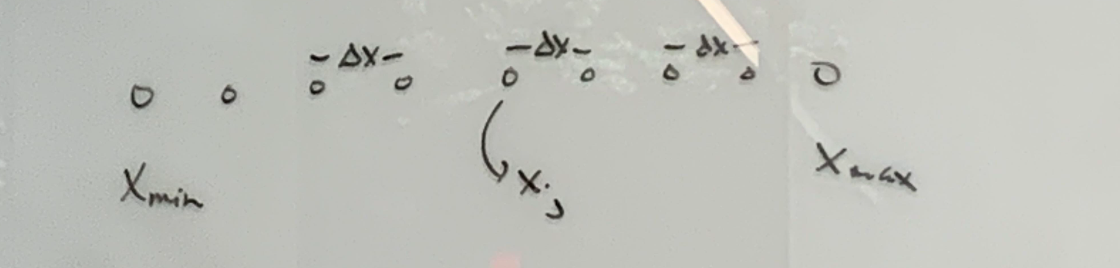
\includegraphics[width = 0.9 \linewidth]{Images/410_discretizationstep.png}


    $\Delta x$ is constant $\rightarrow$ uniform

    \item Grid function notation: $\qquad f(x_j) = f_j$
    \item number of grid points $M_x$

    \item Mesh spacing 

    \[ \Delta x = \frac{x_{max}-x_{min}}{M_x - 1}\]

    Grid points $x_j$

    \[ x_j = x_{min} + (j-1) \Delta x \qquad j = 1,2,...,M_x\]

\end{itemize}

\textbf{Sept 22nd 2023}

\subsubsection{Discretization: Step 2 - derivation of FDAs}

\begin{enumerate}
    \item 3 for first deriv
    \item 1 for 2nd deriv
\end{enumerate}

\begin{itemize}
    \item First, write down, demonstrate accuracy; later derivation
    \item independent variable doesn't matter (use y)
\end{itemize}

\textbf{4.1 First Order, Forward FDA for 1st derivative f'(x)}

\[ f'(x) \approx \frac{f(x+\Delta x)-f(x)}{\Delta X}\]

Note Use a value "forward" of x.

\begin{itemize}
    \item Grid function notation

    \[ f_j' \equiv f'(x_j) \approx \frac{f_{j+1} - f_j}{\Delta x}\]

    \begin{equation}
        f'(x_j) \rightarrow \frac{f_{j+1}-f_j}{\Delta x} \qquad \text{Where the arrow represents "Gets replaced with"}
    \end{equation}

    \item Accuracy?

    \item use taylor series $h\rightarrow\Delta x$ in (TS)

    \[f(x+\Delta x) = f(x) + \Delta x f'(x) + \frac{1}{2} \Delta x^2 f''(x) + \frac{1}{6} \Delta x^3 f'''(x) + O(\Delta x^4) \]

    \item From equation above we have 

    \[ \frac{f(x+\Delta x)-f(x)}{\Delta x} = f'(x) + \frac{1}{2} \Delta x f''(x) + \frac{1}{6} + \Delta x^2 f'''(x) + O(\Delta x^3)\]

    \[ =  f'(x) + \frac{1}{2} \Delta x f''(x) + O(\Delta x^2)\]

    Note: Leading order truncation error is the f''(x) term

    \[ f'(x) + O(\Delta x)\]

    \item Error term $ O(\Delta x) $ means we have first order accurate approx. for the deriv of f(x) at x.

    \item i.e. as $\Delta x \rightarrow 0 $, error in approximation will tend to decrease linearly in $\Delta x$; e.g. as $\Delta x \rightarrow/2 $ we also get error $\rightarrow$ error/2
    
\end{itemize}

\textbf{4.2 First Order Backward FDA for 1st derivative f'(x)}

\[ f'(x) \approx \frac{f(x)-f(x-\Delta x)}{\Delta x}\]

\[ f_j' \equiv f'(x_j) \approx \frac{f_j-f_{j-1}}{\Delta x}\]

\begin{equation}
    f'(x_j) \rightarrow \frac{f_j-f_{j-1}}{\Delta x}
\end{equation}

\begin{itemize}
    \item Accuracy
    \item Again, use Taylor Series

    \[ f(x-\Delta x) = f(x) - \Delta x f'(x) + \frac{\Delta x^2}{2} f''(x) - \frac{\Delta x^3}{6} f'''(x) + O(\Delta x^4)\]

    put equation above into this one

    \[ \frac{f(x)-f(x-\Delta x)}{\Delta x} = f'(x) - \frac{1}{2} \Delta x f''(x) + O(x^2)\]

    \[ = f'(x) + O(x^2)\]
\end{itemize}

\textbf{4.3 Second Order Centred FDA for first derivative f'(x)}

\begin{itemize}
    \item intuitively, taking average of forward, backward should increase accuracy
    \item try:

    \[ \frac{1}{2} \left( \frac{f(x+\Delta x)-f(x)}{\Delta x} + \frac{f(x)-f(x-\Delta x)}{\Delta x} \right)\]

    \[ = \frac{f(x+\Delta x) - f(x-\Delta x)}{2 \Delta x}\]
 
    \begin{equation}
        f'(x_j) \rightarrow \frac{f_{j+1} - f_{j-1}}{2\Delta x}
    \end{equation}
    \item Accuracy

    \[ f(x+\Delta x) = f(x) + \Delta x f'(x) + \frac{1}{2} \Delta x^2 f''(x) + \frac{1}{6} \Delta x^3 f'''(x) + O (\Delta x^4) \]

    \[ f(x-\Delta x) = f(x) - \Delta xf'(x) + \frac{1}{2}\Delta x^2f''(x) - \frac{1}{6} \Delta x^3 f'''(x) + O(\Delta x^4)\]

    Subtract them and lots cancels out

    \[ \frac{f(x+ \Delta x)-f(x-\Delta x)}{2\Delta x} = f'(x) + \frac{1}{6} \Delta x^3 f'''(x) + O(\Delta x^4)\]

    \[ = f'(x) + O(\Delta x^2)\]

    Second order accuracy

    \item  e.g. as $\Delta x \rightarrow \Delta x/2 \qquad \text{we find error} \rightarrow \text{error}/4$

    \item approximation is called "centred"; structure of formula is symmetric about $x_j$
\end{itemize}

\textbf{4.4 Second Order Centred Diff. Approx for f''(x)}

\begin{itemize}
    \item claim: Following is $O(\Delta x^2)$ approx of f''(x)

    \[ f''(x) \approx \frac{f(x+\Delta x) - 2f(x) + f(x-\Delta x)}{\Delta x^2}\]

    \begin{equation}
        f''(x_j) \rightarrow \frac{f_{j+1}-2 f_j + f_{j-1}}{\Delta x^2}
    \end{equation}

    \item Justification: Use Taylor Series

    \[f(x-\Delta x) = f(x) - \Delta x f'(x) + \frac{\Delta x^2}{2} f''(x) - \frac{\Delta x^3}{6} f'''(x) + \frac{\Delta x^4}{24} f''''(x) + O (\Delta x^5)\]

    \[-2f(x) = -2 f(x)\]

    \[ f(x+\Delta x) = f(x) + \Delta x f'(x) + \frac{\Delta x^2}{2} f''(x) + \frac{\Delta x^3}{6} f'''(x) + \frac{\Delta x^4}{24} f''''(x) + O(\Delta x^5)\]

    Subtract terms (reverse engineering style to try to get back to claimed equation)

    \[\frac{f(x+\Delta x) - 2f(x) + f(x-\Delta x)}{\Delta x^2} = f''(x) + \frac{\Delta x^2}{12} f''''(x) + O(\Delta x^4) \]
    \[ = f''(x) + O(\Delta x^2)\]

    Second order error term (as claimed)
    
\end{itemize}


\subsection{Deriving FDAs using taylor series (exam hint)}
\begin{itemize}
    \item Need to choose points that will be used in FDA

    \[ . \qquad . \qquad . \qquad . \qquad . \qquad . \qquad . \qquad . \qquad . \qquad . \qquad . \qquad . \qquad \]

    $x_{j-1}, \qquad x_j, \qquad  x_{j+1}$

    \item Example: Determine approximation to f''(x) that uses $x_j, x_{j+1}, x_{j-1}$

    \item Assume that an appropriate linear combination of truncated taylor series for $f_{j-1}$, $f_j$, $f_{j+1}$ will give the formula 

    \[ \rightarrow \text{consider:} \]
    
    \begin{equation}
        \alpha f_{j-1} + \beta f_j + \gamma f_{j+1} = f''(x) + ...
    \end{equation}

    \item Taylor expanding 

    \[ f_{j-1} = f(x-\Delta x) = f(x) - \Delta xf'(x)+ \frac{1}{2} \Delta x^2 f''(x) - \frac{\Delta x^3}{6} f'''(x) + O(\Delta x^4)\]

    \[ f_j = f(x)\]

    \[ f_{j+1} = f(x+\Delta x) = f(x) + \Delta xf'(x)+ \frac{1}{2} \Delta x^2 f''(x) + \frac{\Delta x^3}{6} f'''(x) + O(\Delta x^4)\]

    \item Now require equation give f''(x) at leading order

    \[ \alpha + \beta + \gamma = 0 \qquad \text{(No f(x) term)}\]
    \[ -\alpha  + \gamma = 0 \qquad \text{(No f'(x) term)}\]
    \[\frac{\Delta x^2}{2}(\alpha + \gamma)=1 \qquad \text{(Gives us f''(x))}\]

    \item Solving

    \[\alpha = \frac{1}{\Delta x^2}\]

    \[ \beta = \frac{-2}{\Delta x^2}\]

    \[ \gamma = \frac{1}{\Delta x^2}\]

    \item So our FDA is 

    \[ f''(x_j) \rightarrow \frac{f_{j+1}-2f_j + f_{j-1}}{\Delta x^2}\]
    
\end{itemize}


problem hint for exam

\subsection{Canonical method for specifying grid spacing (nuts and bolts topic)}

\[ . \qquad . \qquad . \qquad . \qquad . \qquad . \qquad . \qquad . \qquad . \qquad . \qquad . \qquad . \qquad \]

Mesh (partial) grid with each dot separated by $\Delta x$

\vspace{10 px}

Nothing special about spacing, so we can change it if we want...?

\begin{itemize}
    \item Whenever solving DE's with FDA, change $\Delta x$ to see what happens 
    \item Changes by a factor of 2 are most convenient
    \[ \Delta x, \Delta x/2, \Delta x/4, \Delta x/8 ...\]

    \[ l , l+1, l+2, l+3\]

    \item Discretization parameter: Level l

    \[ n_x = 2^l + 1\]

    \[ \Delta x = \frac{x_{max}-x_{min}}{2^l}\]

    Just easier to think/specify in terms of l.

    \item Very small values of l not likely to be of much use; more likely to use $ l = 6,7,8,...$ corresponding to $n_x = 65,129,257,...$

    \item As $l$ and $n_x$ get larger, $\Delta x$ gets smaller and FDA should become more accurate.
\end{itemize}

\subsection{Richardson Extrapolation}
\begin{itemize}
    \item Basic Idea: FD approximation using different scales of discretization $\Delta x_1,\Delta x_2,\Delta x_3,...$ but the same F.D. template $\rightarrow$ combine to get higher order approximation.
    \item Example: Forward approx. of first derivative
    \item Recall

    \[ L^{\Delta x} f = \frac{f(x+\Delta x)+f(x)}{\Delta x} = f'(x) + \frac{1}{2} \Delta x f''(x)+ \frac{1}{6} \Delta x^2 f'''(x) + O(\Delta x^3)\]

    \[ L^{2\Delta x} f = \frac{f(x+2\Delta x)+f(x)}{2\Delta x} = f'(x) + \frac{1}{2} 2\Delta x f''(x)+ \frac{1}{6} 2\Delta x^2 f'''(x) + O(\Delta x^3)\]

    \item Take linear combination

    \[ \alpha L^{\Delta x} f+ \beta l^{2\Delta x} f = f'(x) + O(\Delta x^2)\]

    So giving us

    \[ \alpha + \beta = 1 \]

    \[ \alpha + 2\beta = 0 \]

    ("again this sort of thing is Good for exam purposes again")

    \item Solve 2 equations 

    \[ \alpha = 2\]

    \[ \beta = -1 \]

    giving us

    \[ \alpha L^{\Delta x} f+ \beta l^{2\Delta x} f = s\left( \frac{f_{j+1}-f_j}{\Delta x}\right) - \left(\frac{f_{j+2}-f_j}{2 \Delta x}\right) \]

    

    \[ \rightarrow \qquad \frac{1f_{j+2}+4f_{j+1}-3f_j}{2\Delta x}\]

    \[ = f'(x) - \frac{1}{3} \Delta x^2 f'''(x) + O (\Delta x^3) = f'(x) + O(\Delta x^2)  \]

    \item Can linear combination of 3,4,... approximations to constant even more accurate formulae
    
    
\end{itemize}
